\documentclass[11pt]{article}
\usepackage[english]{babel}
\usepackage[utf8]{inputenc}
\usepackage[margin=0.5in]{geometry}
\usepackage{amsmath}
\usepackage{amsthm}
\usepackage{amsfonts}
\usepackage{amssymb}
\usepackage[usenames,dvipsnames]{xcolor}
\usepackage{graphicx}
\usepackage[siunitx]{circuitikz}
\usepackage{tikz}
\usepackage[colorinlistoftodos, color=orange!50]{todonotes}
\usepackage{hyperref}
\usepackage[numbers, square]{natbib}
\usepackage{fancybox}
\usepackage{epsfig}
\usepackage{soul}
\usepackage[framemethod=tikz]{mdframed}
\usetikzlibrary{positioning, automata, backgrounds}
\usepackage[shortlabels]{enumitem}
\usepackage[version=4]{mhchem}
\usepackage{multicol}
\usepackage{forest}
\usepackage{mathtools}
\usepackage{comment}
\usepackage{enumitem}
\usepackage[utf8]{inputenc}
\usepackage[linesnumbered,ruled,vlined]{algorithm2e}
\usepackage{listings}
\usepackage{color}
\usepackage[numbers]{natbib}
\usepackage{subfiles}
\usepackage{tkz-berge}


\newcommand{\interval}[4]{\draw (#2, #1) -- (#3, #1); % Usage: \interval{height}{start}{end}{label}
\draw (#2, #1-0.11) -- (#2, #1+0.11); % draw left whisker
\draw (#3, #1-0.11) -- (#3, #1+0.11); % draw right whisker
\node[] at (#2-0.25, #1) {#4};
}

\newtheorem{prop}{Proposition}[section]
\newtheorem{thm}{Theorem}[section]
\newtheorem{lemma}{Lemma}[section]
\newtheorem{cor}{Corollary}[prop]

\theoremstyle{definition}
\newtheorem{definition}{Definition}

\theoremstyle{definition}
\newtheorem{required}{Problem}

\theoremstyle{definition}
\newtheorem{ex}{Example}


\setlength{\marginparwidth}{3.4cm}
%#########################################################

%To use symbols for footnotes
\renewcommand*{\thefootnote}{\fnsymbol{footnote}}
%To change footnotes back to numbers uncomment the following line
%\renewcommand*{\thefootnote}{\arabic{footnote}}

% Enable this command to adjust line spacing for inline math equations.
% \everymath{\displaystyle}

% _______ _____ _______ _      ______ 
%|__   __|_   _|__   __| |    |  ____|
%   | |    | |    | |  | |    | |__   
%   | |    | |    | |  | |    |  __|  
%   | |   _| |_   | |  | |____| |____ 
%   |_|  |_____|  |_|  |______|______|
%%%%%%%%%%%%%%%%%%%%%%%%%%%%%%%%%%%%%%%

\title{
\normalfont \normalsize 
\textsc{CSCI 3104 Spring 2023 \\ 
Instructors: Prof. Layer and Chandra Kanth Nagesh} \\
[10pt] 
\rule{\linewidth}{0.5pt} \\[6pt] 
\huge Homework 3 \\
\rule{\linewidth}{2pt}  \\[10pt]
}
%\author{}
\date{}

\begin{document}

\definecolor {processblue}{cmyk}{0.96,0,0,0}
\definecolor{processred}{rgb}{200, 0, 0}
\definecolor{processgreen}{rgb}{0, 255, 0}
\DeclareGraphicsExtensions{.png}
\DeclareGraphicsExtensions{.gif}
\DeclareGraphicsExtensions{.jpg}

\maketitle


%%%%%%%%%%%%%%%%%%%%%%%%%
%%%%%%%%%%%%%%%%%%%%%%%%%%
%%%%%%%%%%FILL IN YOUR NAME%%%%%%%
%%%%%%%%%%AND STUDENT ID%%%%%%%%
%%%%%%%%%%%%%%%%%%%%%%%%%%
\noindent
Due Date \dotfill February 9, 2023 \\
Name \dotfill \textbf{Blake Raphael} \\
Student ID \dotfill \textbf{109752312} \\
Collaborators \dotfill \textbf{Alex Barry, Brody Cyphers, and Ben Kohav}

\tableofcontents

\section{Instructions}
 \begin{itemize}
	\item The solutions \textbf{should be typed}, using proper mathematical notation. We cannot accept hand-written solutions. \href{http://ece.uprm.edu/~caceros/latex/introduction.pdf}{Here's a short intro to \LaTeX.}
	\item You should submit your work through the \textbf{class Gradescope page} only (linked from Canvas). Please submit one PDF file, compiled using this \LaTeX \ template.
	\item You may not need a full page for your solutions; pagebreaks are there to help Gradescope automatically find where each problem is. Even if you do not attempt every problem, please submit this document with no fewer pages than the blank template (or Gradescope has issues with it).

	\item You are welcome and encouraged to collaborate with your classmates, as well as consult outside resources. You must \textbf{cite your sources in this document.} \textbf{Copying from any source is an Honor Code violation. Furthermore, all submissions must be in your own words and reflect your understanding of the material.} If there is any confusion about this policy, it is your responsibility to clarify before the due date. 

	\item Posting to \textbf{any} service including, but not limited to Chegg, Reddit, StackExchange, etc., for help on an assignment is a violation of the Honor Code.

	\item You \textbf{must} virtually sign the Honor Code (see Section \ref{HonorCode}). Failure to do so will result in your assignment not being graded.
\end{itemize}


\section{Honor Code (Make Sure to Virtually Sign)} \label{HonorCode}

%\begin{required}
\begin{itemize}
\item My submission is in my own words and reflects my understanding of the material.
\item Any collaborations and external sources have been clearly cited in this document.
\item I have not posted to external services including, but not limited to Chegg, Reddit, StackExchange, etc.
\item I have neither copied nor provided others solutions they can copy.
\end{itemize}

%\noindent In the specified region below, clearly indicate that you have upheld the Honor Code. Then type your name. 
%\end{required}

\begin{proof}[Agreed (I agree to the above, Blake Raphael).]
%% Typing "I agree to the above," followed by your name is sufficient.
\end{proof}

\newpage
\section{Standard 3 - Dijkstra's Algorithm}

\subsection{Problem \ref{Dijkstra0} (1 point)}
\begin{required} \label{Dijkstra0}
Consider the weighted graph $G(V, E, w)$ pictured below. Work through Dijkstra's algorithm on the following graph, using the source vertex $E$. 
\begin{itemize}
\item Clearly include the contents of the priority queue, as well as the distance from $E$ to each vertex at each iteration.
\item If you use a table to store the distances, clearly label the keys according to the vertex names rather than numeric indices (i.e., \texttt{dist[`B']} is more descriptive than \texttt{dist[`1']}).
\item You do \textbf{not} need to draw the graph at each iteration, though you are welcome to do so. [This may be helpful scratch work, which you do not need to include.]
\end{itemize}


\begin{center}
\begin {tikzpicture}[-latex, auto, node distance =2 cm and 3cm, semithick]
\tikzstyle{blue}=[circle ,top color =white , bottom color = processblue!20 ,draw,processblue , text=blue , minimum width =1 cm];
\tikzstyle{red}=[circle ,top color =white , bottom color = processred!20 ,draw, processred , text=blue , minimum width =1 cm];
\tikzstyle{green}=[circle ,top color =white , bottom color = processgreen!20 ,draw, processgreen , text=blue , minimum width =1 cm];

	\node[blue] (A) {$A$};
	\node[blue] (C) [below right = of A] {$C$};
	\node[blue] (B) [below right = of C] {$B$};
	\node[blue] (E) [below left = of A] {$E$};
	\node[blue] (D) [below left = of E] {$D$};
	\node[blue] (H) [below right = of D] {$H$};
	\node[blue] (F) [right = of H] {$F$};

	\path (A) edge node[above] {$2$}  (C);
	\path (E) edge node[left]  {$6$}  (A);

	\path (C) edge node[above] {$1$}  (B);
	\path (B) edge node[below] {$5$}  (F);

	\path (E) edge node[above] {$3$} (C);
	\path (C) edge node[above] {$4$}  (F);

	\path (D) edge node[above] {$8$}  (H);

	\path (E) edge node[above] {$11$} (F);
	\path (E) edge node[right] {$6$}  (D);
	\end{tikzpicture}  
\end{center}

\end{required}

\begin{proof}[Answer]
\indent The following block will outline the priority queue step-by-step:
\begin{table}[h!]
	\begin{center}
		\caption{Priority Queue Contents}
		\label{tab:table1}
		\begin{tabular}{l|c|r} % <-- Alignments: 1st column left, 2nd middle and 3rd right, with vertical lines in between
			\textbf{Step} & \textbf{Queue Contents} & \textbf{Distance}\\
			\hline
			0 & E & N/A\\
			1 & C & 3\\
			2 & C, A & 3, 6\\
			3 & C, A, D & 3, 6, 6\\
			4 & C, A, D, F & 3, 6, 6, 11\\
			5 & B, A, D, F & 4, 6, 6, 11\\
			6 & B, A, D, F & 4, 6, 6, 7\\
			7 & A, D, F & 6, 6, 7\\
			8 & D, F & 6, 7\\
			9 & F, H & 7, 14\\
			10 & H & 14\\
			11 & All Nodes Explored & All Nodes Explored\\
		\end{tabular}
	\end{center}
\end{table}

\begin{table}[h!]
	\begin{center}
		\label{tab:table1}
		\begin{tabular}{l|r} % <-- Alignments: 1st column left, 2nd middle and 3rd right, with vertical lines in between
			\textbf{Node} & \textbf{Final Distance From E}\\
			\hline
			A & 6 \\
			B & 4 \\
			C & 3 \\
			D & 6 \\
			F & 7 \\
			H & 14 \\
		\end{tabular}
	\end{center}
\end{table}
\end{proof}

\newpage
\subsection{Problem \ref{Dijkstra2}} 
\begin{required} \label{Dijkstra2}
You have three batteries, with capacities of 20, 15, and 8 Ah (Amp-hours), respectively. The 15 and 8-Ah batteries are fully charged (containing 15 Ah and 8 Ah, respectively), while the 20-Ah battery is empty, with 0 Ah. You have a battery transfer device which has a ``source'' battery position and a ``target'' battery position. When you place two batteries in the device, it instantaneously transfers as many Ah from the source battery to the target battery as possible. Thus, this device stops the transfer either when the source battery has no Ah remaining or when the destination battery is fully charged (whichever comes first).  \\

\noindent But battery transfers aren't free! The battery device is also hooked up to your phone by bluetooth, and automatically charges you a number of dollars equal to however many Ah it just transfered.  \\
	
\noindent The goal in this problem is to determine whether there exists a sequence of transfers that leaves exactly 5 Ah either in the 15-Ah battery or the 8-Ah battery, and if so, how little money you can spend to get this result. \\

\noindent Do the following.
\begin{enumerate}[label=(\alph*)]
\subsubsection{Problem 2\ref{Dijkstra2a} (1 point)}
\item \label{Dijkstra2a} Rephrase this is as a graph problem. Give a precise definition of how to model this problem as a graph, and state the specific question about this graph that must be answered. [\textbf{Note:} While you are welcome to draw the graph, it is enough to provide 1-2 sentences clearly describing what the vertices are and when two vertices are adjacent. If the graph is weighted, clearly specify what the edge weights are.]

\begin{proof}[Answer]
We will consider each node as a state space with the values of each battery. Each edge represents a single transfer between batteries, changing the state. When two nodes are adjacent and connected with an edge, there was a transfer between those batteries. Each edge weight represents the cost of the transfer.
\end{proof}

\newpage
\subsubsection{Problem 2\ref{Dijkstra2b} (1 point)}
\item \label{Dijkstra2b} Clearly describe an algorithm to solve this problem. If you use an algorithm covered in class, it is enough to state that. If you modify an algorithm from class, clearly outline any modifications. Make sure to explicitly specify any parameters that need to be passed to the initial function call.

\begin{proof}[Answer]
We will be using Dijkstra's algorithm to find the shortest weighted path, which gives us the lowest cost.
\end{proof}



\newpage
\subsubsection{Problem 2\ref{Dijkstra2c} (1 point)}
\item \label{Dijkstra2c} Apply that algorithm to the question. Report and justify your answer. Here, justification includes the sequences of vertices visited and the total cost. 

\begin{proof}[Answer]
When we use Dijkstra's algorithm, we get the following sequence of nodes to our final cost:\\

\begin{center}
	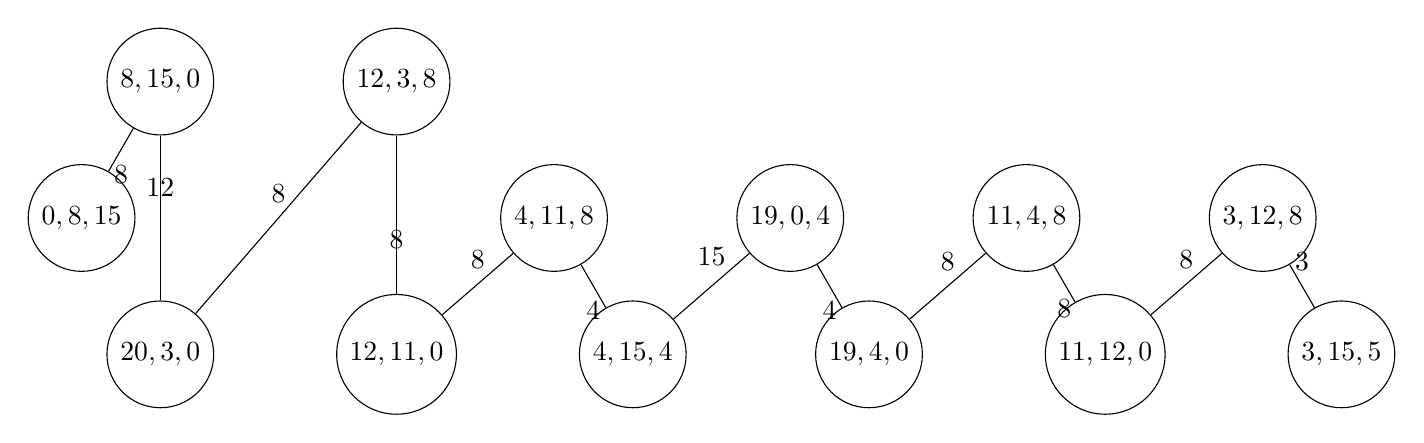
\begin{tikzpicture}[
		wide/.style={line width=4pt},
		every node/.style={circle,draw,minimum size=16},
		scale=2]
		\node (1) at (-0.5,0)            {$0,8,15$};
		\node (2) at ($ (1) + ( 60:1)$) {$8,15,0$};
		\node (3) at ($ (1) + (-60:1)$) {$20,3,0$};
		\node (4) at ($ (2) + ( 1.5,0 )$) {$12,3,8$};
		\node (5) at ($ (3) + ( 1.5,0 )$) {$12,11,0$};
		\node (6) at ($ (4) + (-60:1) + (0.5,0)$) {$4,11,8$};
		\node (7) at ($ (5) + ( 1.5,0 )$) {$4,15,4$};
		\node (8) at ($ (6) + ( 1.5,0 )$) {$19,0,4$};
		\node (9) at ($ (7) + ( 1.5,0 )$) {$19,4,0$};
		\node (10) at ($ (8) + ( 1.5,0 )$) {$11,4,8$};
		\node (11) at ($ (9) + ( 1.5,0 )$) {$11,12,0$};
		\node (12) at ($ (10) + ( 1.5,0 )$) {$3,12,8$};
		\node (13) at ($ (11) + ( 1.5,0 )$) {$3,15,5$};
		\draw (1) -- node[below, draw=none,fill=none]{8}(2);
		\draw (2) -- node[above, draw=none,fill=none]{12}(3);
		\draw (3) -- node[above, draw=none,fill=none]{8}(4);
		
		% Replace the line \draw (w) -- (t); with the line below (after deleting the % symbol to uncomment) in order to draw a thicker edge.
		%		\draw[line width=3pt] (w) -- (t);
		
		
		\draw (4) -- node[below, draw=none,fill=none]{8}(5);
		\draw (5) -- node[above, draw=none,fill=none]{8}(6);
		\draw (6) -- node[below, draw=none,fill=none]{4}(7);
		\draw (7) -- node[above, draw=none,fill=none]{15}(8);
		\draw (8) -- node[below, draw=none,fill=none]{4}(9);
		\draw (9) -- node[above, draw=none,fill=none]{8}(10);
		\draw (10) -- node[below, draw=none,fill=none]{8}(11);
		\draw (11) -- node[above, draw=none,fill=none]{8}(12);
		\draw (12) -- node[above, draw=none,fill=none]{3}(13);
		
	\end{tikzpicture}
\end{center}

The final cost of the transfers is $94$.\\
\end{proof}

\end{enumerate}
\end{required}



\end{document} % NOTHING AFTER THIS LINE IS PART OF THE DOCUMENT



